\documentclass[a4paper,12pt]{article}
%
% Demo of the mcode package from 
% http://www.mathworks.co.uk/matlabcentral/fileexchange/8015-m-code-latex-package
% Updated 06 Mar 2014
%

%Packages for portuguese
\usepackage[brazilian]{babel}
% ---
% Para problemas de acento descomente (apenas) uma das linhas abaixo
\usepackage[utf8]{inputenc}
%\usepackage[latin1]{inputenc} 
% ---
\usepackage[T1]{fontenc}

% to include graphics and eps matlab plot
\usepackage{graphicx}
%\usepackage{epstopdf} % just in case to convert eps to pdf
%\graphicspath{{./figs/}} %if the figures are in the subdirectory "figs"

\usepackage[hmargin={2.5cm},vmargin={2.5cm}]{geometry} %setup margins

\usepackage{amssymb,amsmath,amsfonts} %some math packages

% to allow the argument [H] to fix the place of the environments
\usepackage{float}

% load package with ``framed'' and ``numbered'' option.
\usepackage[framed,numbered,autolinebreaks,useliterate]{mcode}

% something NOT relevant to the usage of the package.
\usepackage{url}
\setlength{\parindent}{0pt}
\setlength{\parskip}{18pt}
\title{Exercício Computacional X}
\author{Nome do autor}
\date{\today}
% //////////////////////////////////////////////////

\begin{document}

\maketitle


Segue abaixo os códigos e as saídas geradas para o Exercício X.

\section{Questão 1}

\subsection*{Código Matlab}

Segue o código utilizado na questão.
<copiar e colar o código no ambiente abaixo>
\begin{lstlisting}
%Codigo para gravar no arquivo 'matlabDiary.txt' a saida do codigo
clc;

diary('matlabDiary.txt')

diary on

A = rand(3,3);
A = A + A'
[v,e]=eig(A)

diary off
\end{lstlisting}

<ou, como alternativa, copiar o arquivo matlab .m no diretório do Overleaf e utilizar o comando \verb|\lstinputlisting{/SOME/PATH/FILENAME.M}| ou\\ \verb|\lstinputlisting[firstline=6, lastline=15]{/SOME/PATH/FILENAME.M}| para especificar as linhas>

\medskip

%Specific lines
%\lstinputlisting[firstline=6, lastline=15]{diario.m}

% All lines
\lstinputlisting{diario.m}



\subsection*{Saída gerada pelo código}

Segue a saída gerada:
\begin{lstlisting}

A =

0.7845    1.3615    0.2174
1.3615    0.0637    0.3741
0.2174    0.3741    1.6469


v =

0.6016    0.5300    0.5976
-0.7963    0.3387    0.5012
0.0632   -0.7774    0.6258


e =

-0.9947         0         0
0    1.3357         0
0         0    2.1540
\end{lstlisting}

<A saída também pode ser importada via \verb|\lstinputlisting| para esse documento por meio do arquivo texto \texttt{`matlabDiary.txt'}. O arquivo txt deve estar no diretório do Overleaf>

\lstinputlisting{matlabDiary.txt}


\subsubsection*{Importanto gráficos do Matlab}

Para incluir uma figura Matlab para o documento tex o mais indicado é salvar a figura no formato EPS (formato vetorial) pois não há perda de resolução. Veja um exemplo abaixo de como fazer.
\begin{lstlisting}
x = linspace(0,2*pi);
y = sin(x);
plot(x,y,'o'); xlabel('x'); ylabel('sin(x)'); %plot de figure
print -depsc myfig.eps %save the figure in eps format in the directory of the .m file
\end{lstlisting}

Veja um exemplo na Figura~\ref{fig:theFig}.
\begin{figure}[H]
	\centerline{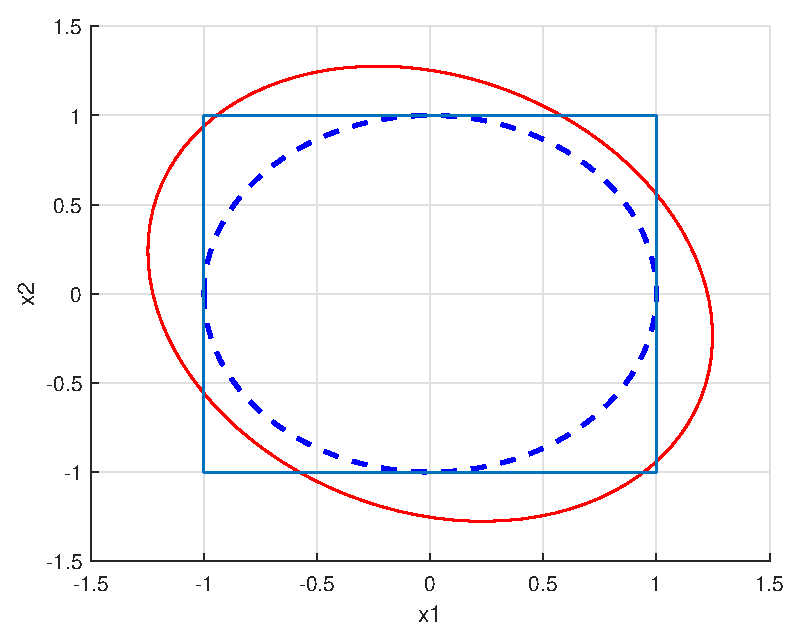
\includegraphics[scale=0.6]{figmatlab}}		
	\caption{My matlab plot. \label{fig:theFig}}
\end{figure}

\end{document}